


\begin{markdown}
#### List of Users
To see a list of people in your organization, click on Organisation in the menu on the left. Users is the first tab.
\end{markdown}

\begin{figure}[h!]
    \centering
    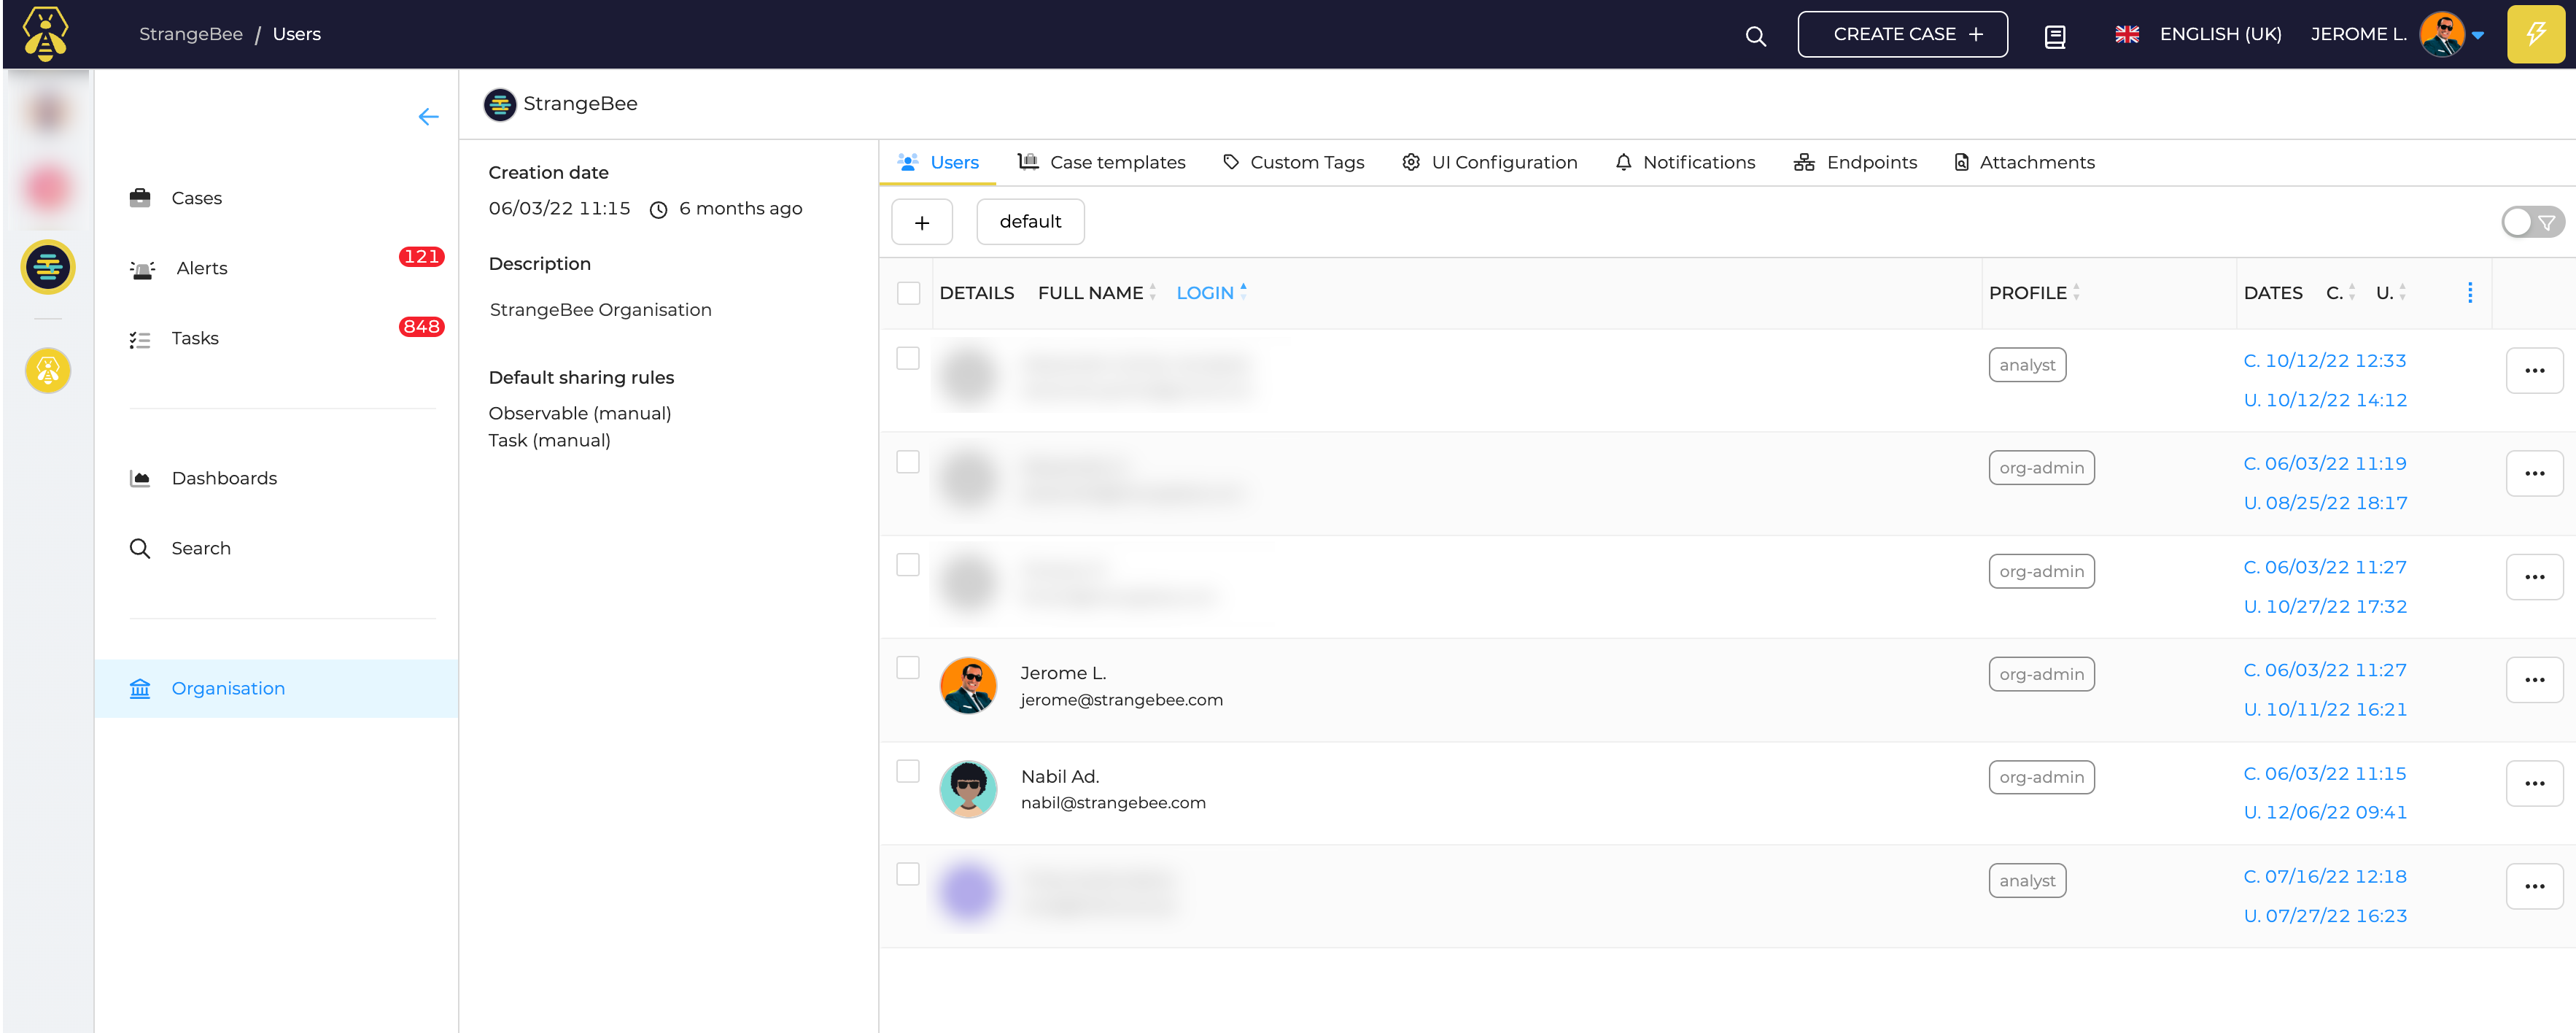
\includegraphics[width=\textwidth]{images/docs/org_admin/manage_users/organisation-list-users.png}
    \caption{List of user accounts}
    \label{fig:modules}
\end{figure}

\begin{markdown}
#### User information
Click the Preview button to see more details about a user.
\end{markdown}

\begin{figure}[H]
    \centering
    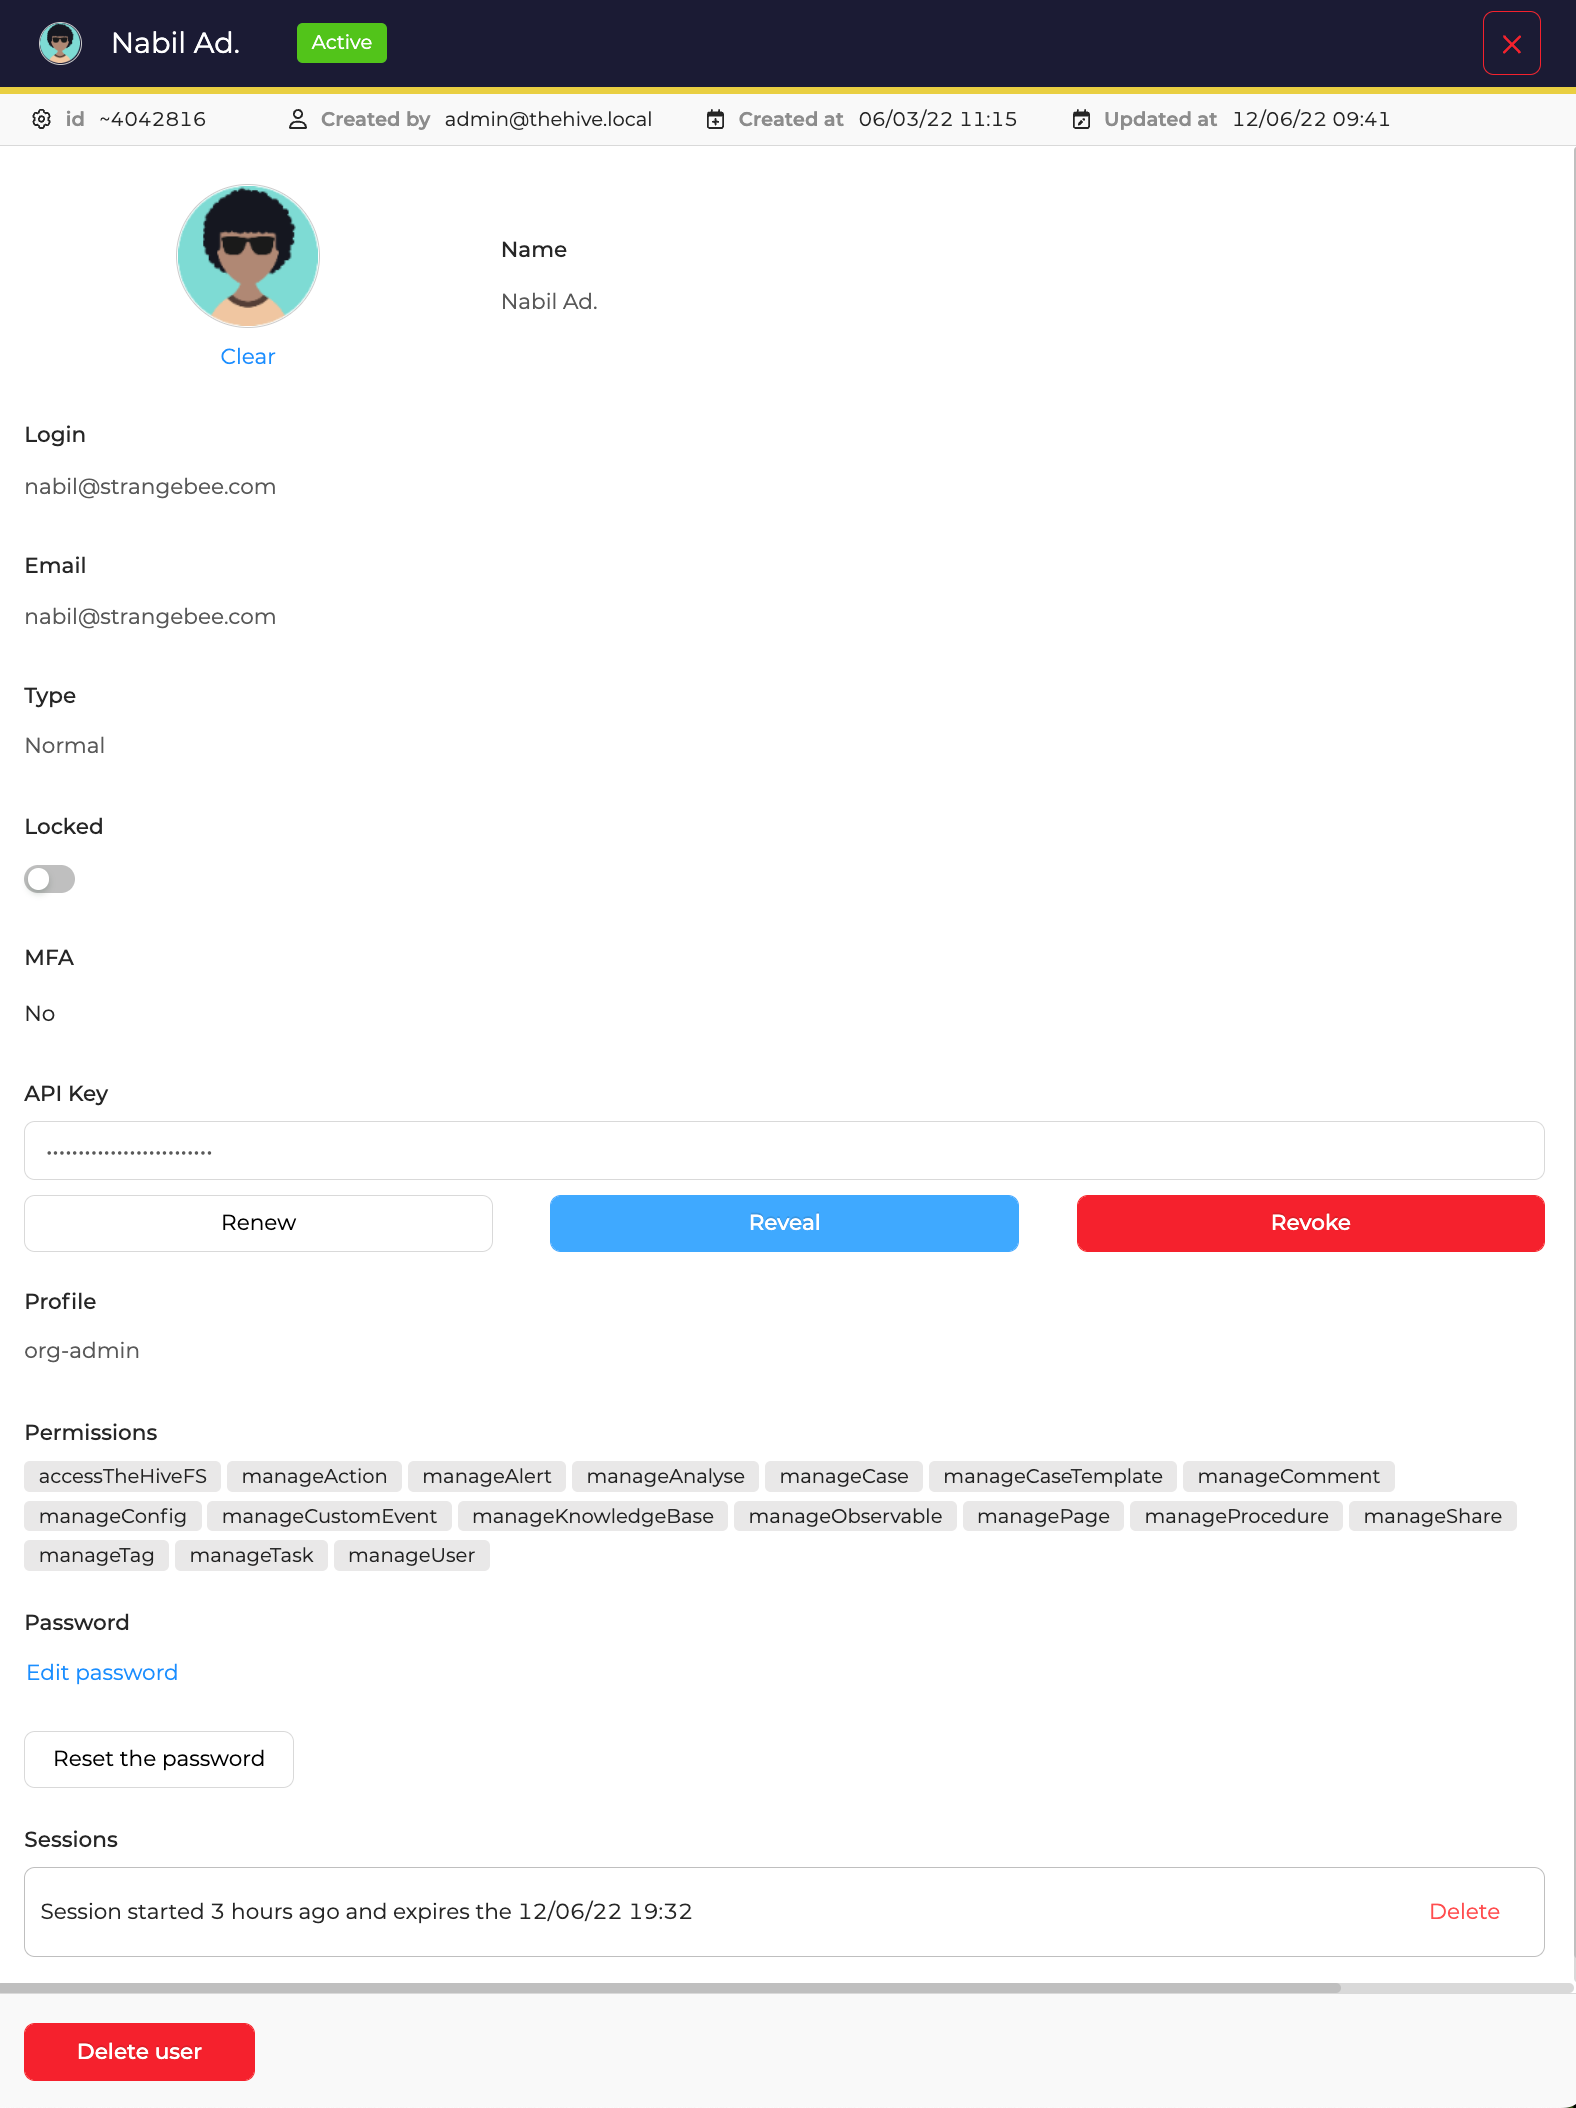
\includegraphics[width=\textwidth]{images/docs/org_admin/manage_users/organisation-user-details.png}
    \caption{User information}
    \label{fig:modules}
\end{figure}

\begin{markdown}
#### Configuration parameters
- __Avatar__ : Update the avatar associated with the user by drag&drop a new file (PNG or JPG files).
- __Login__: User login
- __Email__ : email address for the account. This is used to send notifications or reset password links to users. Login is used if no email is filled there
- __Type__ :
Type of the account. Normal or Service. A Service account cannot open interactive session
- __Locked__ :
Block a user from logging in the application
- __MFA__ :
Tells if a user has configured MFA or not (Multi Factor Authentication). If yes, Yes is displayed
- __API Key__ :
Define, Renew, Reveal or Revoke API key of the account
- __Profile__ :
Information about the profile given to the user
- __Permissions__ :
List of permissions included in the profile
- __Password__ :
Create or update the password of the user
- __Reset Password__ :
If the application is configured with a SMTP server, send an email with a magic link to the user. link is active for a short time period.
- __Sessions__ :
List of opened interactive sessions. Click delete to close a session

#### Add Users
org-admin users or users with the role manageUser in their profile can add users in the current Organisation.
\end{markdown}



\begin{figure}[h!]
    \centering
    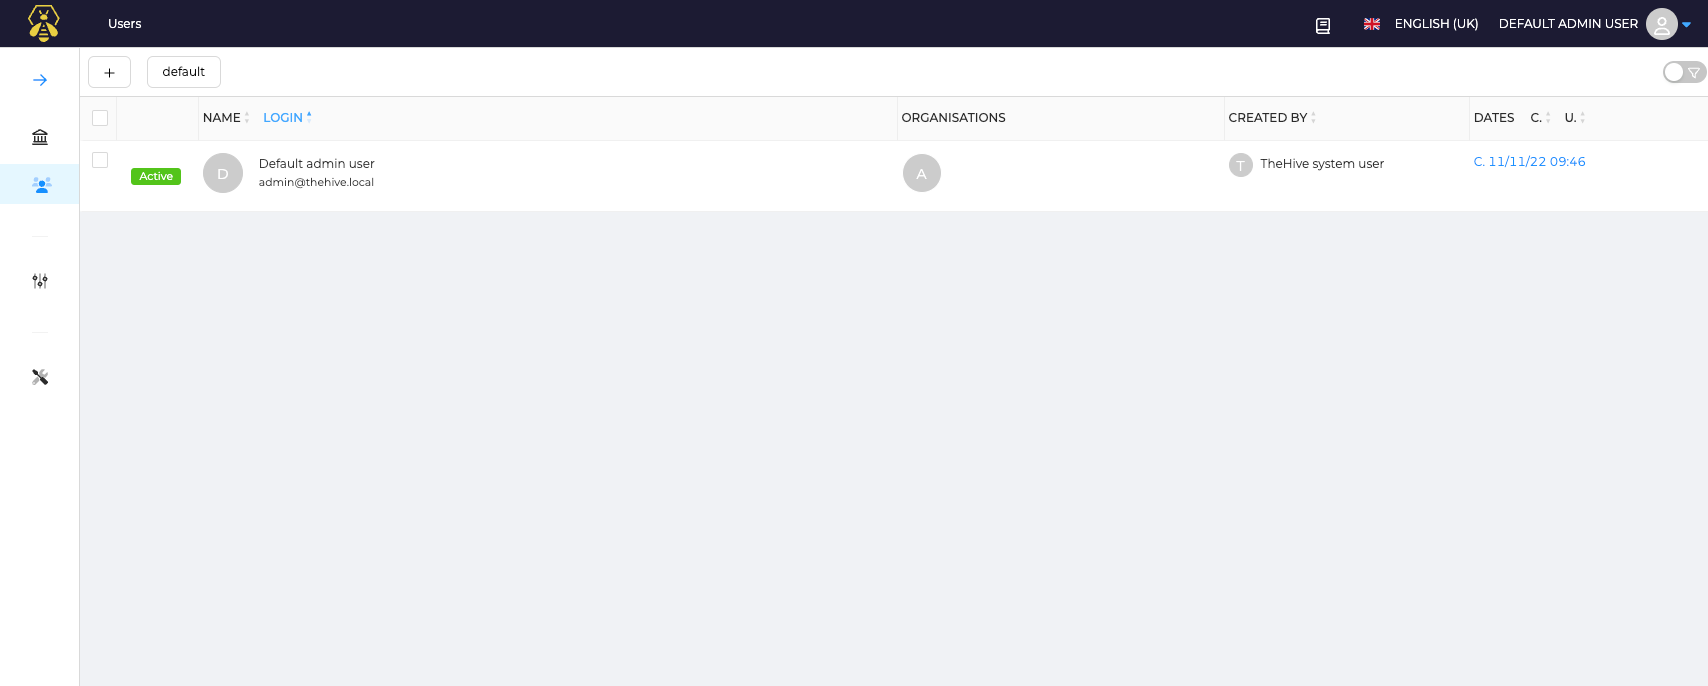
\includegraphics[width=\textwidth]{images/docs/org_admin/manage_users/accounts-1.png}
    \label{fig:modules}
\end{figure}

Click the + button to add an account in the current organisation, and follow create an account and update an account guides.

\begin{figure}[H]
    \centering
    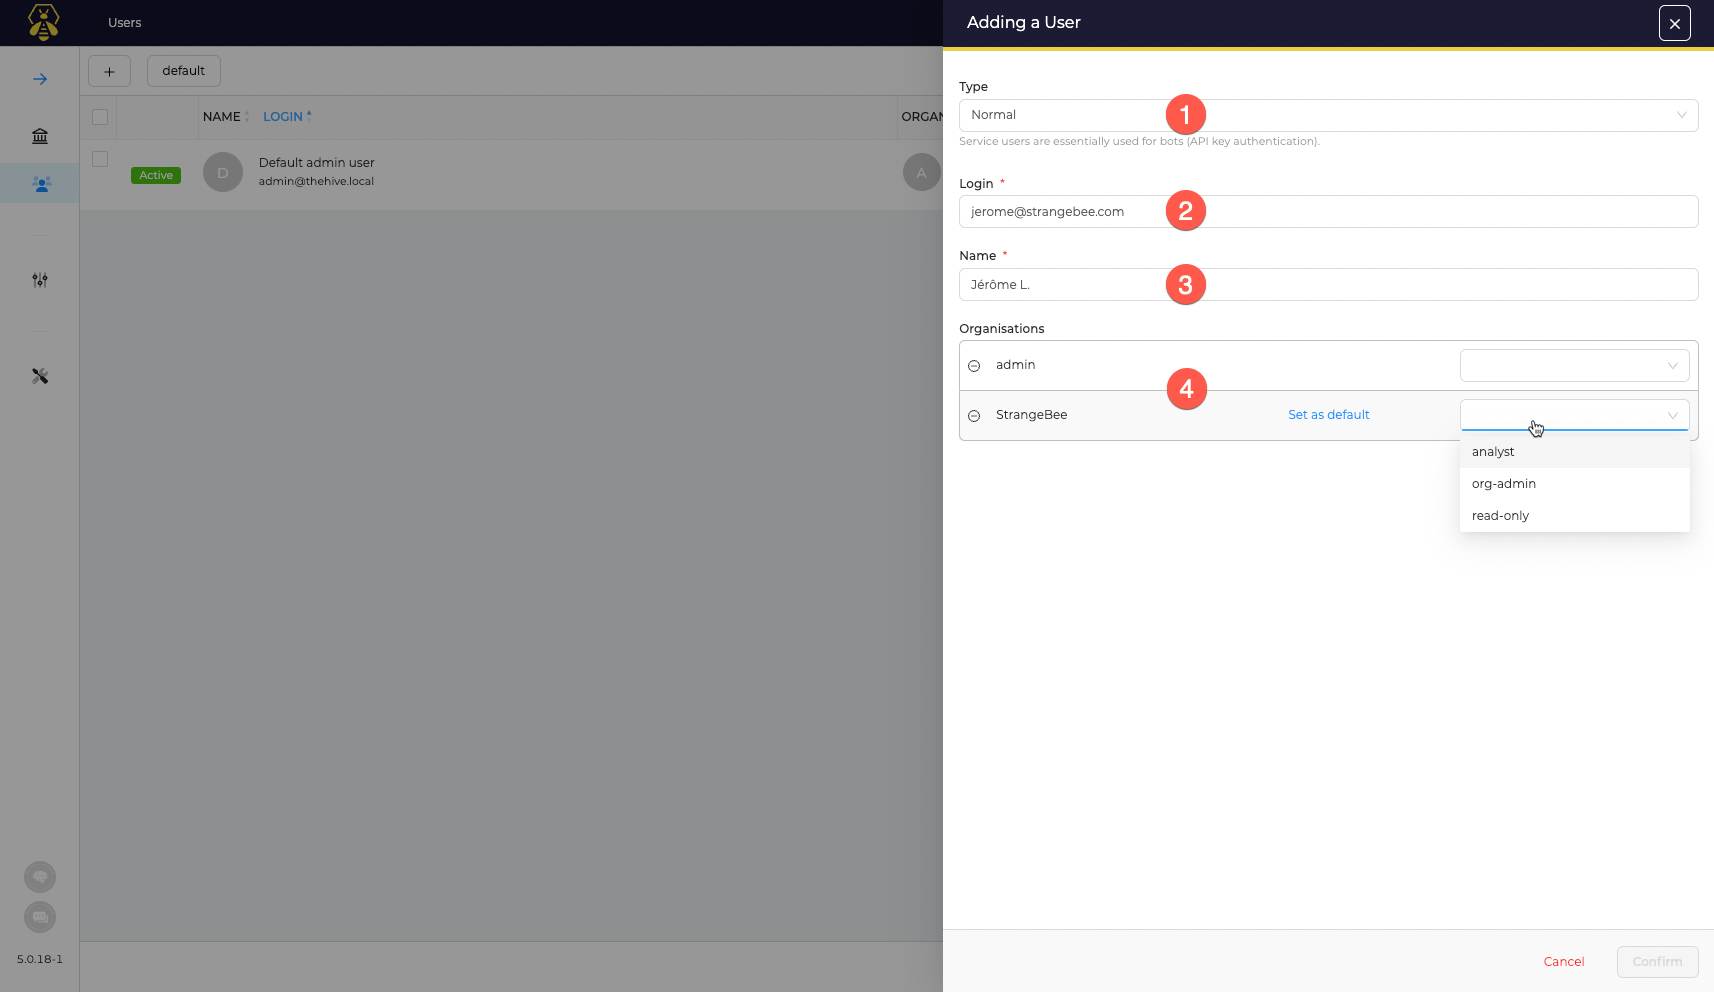
\includegraphics[width=\textwidth]{images/docs/org_admin/manage_users/accounts-2.png}
    \label{fig:modules}
\end{figure}
In the list of accounts, click Preview to open accounts details view.


\begin{figure}[H]
    \centering
    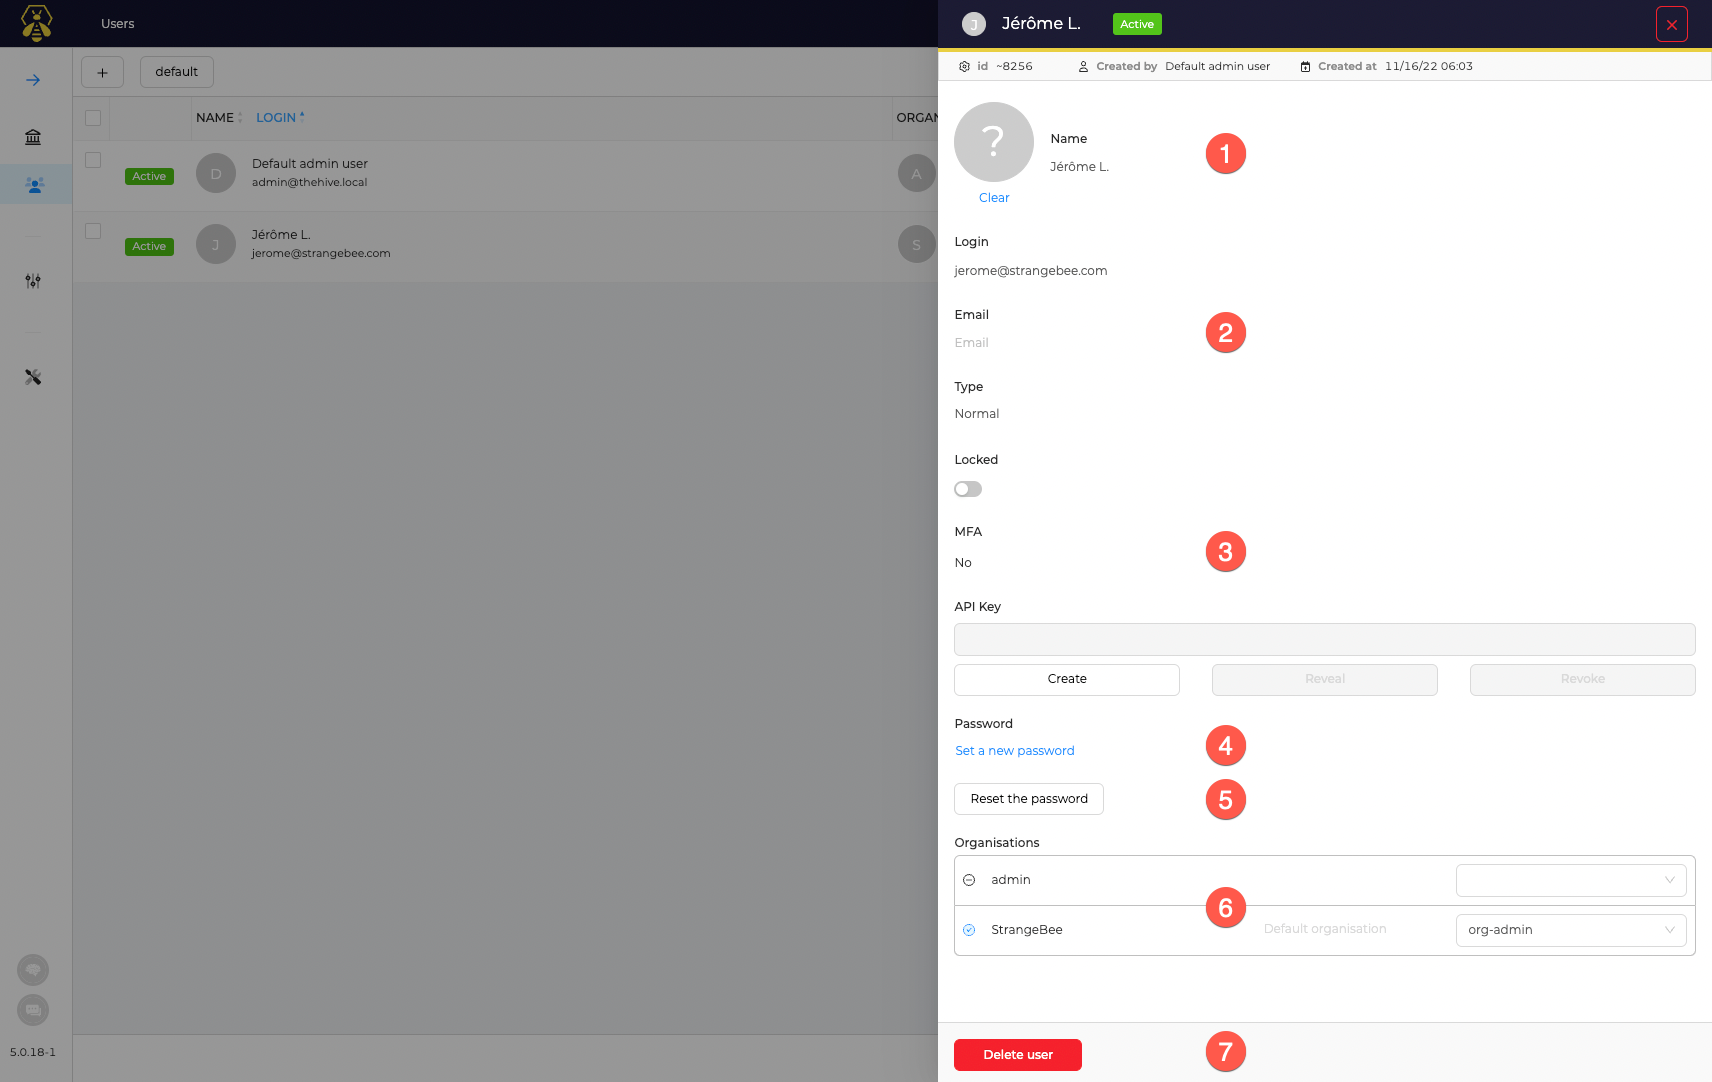
\includegraphics[width=\textwidth]{images/docs/org_admin/manage_users/accounts-3.png}
    \label{fig:modules}
\end{figure}
% \begin{markdown}


% #### User management
% Accounts can be deleted or locked, only in the current organisation.
% \end{markdown}